\textbf{COLUNI 2025 -- Questão 19}\par\medskip Gaia pretende construir uma pipa no formato de um losango e, dentre os materiais necessários, ela precisará de papel de seda e de duas varetas de bambu. Se a figura abaixo representa um esboço do “corpo da pipa”, é CORRETO afirmar que a quantidade de papel de seda necessária, em m$^2$, é igual a:

% COLUNI-AUTO-FIGURES-BEGIN
\begin{figure}[htbp]
\centering
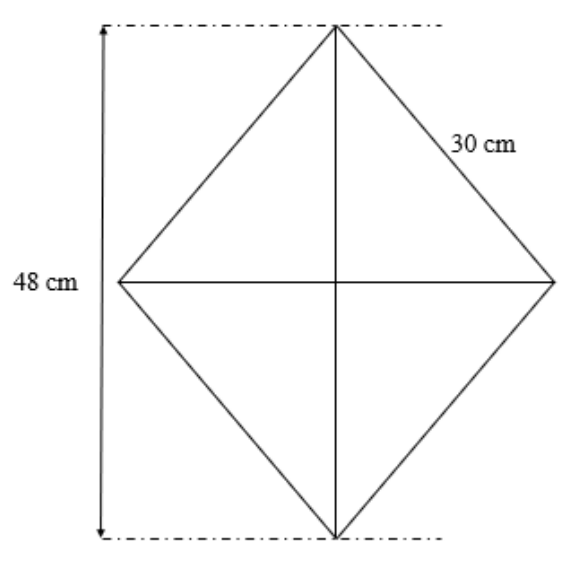
\includegraphics[width=0.7\linewidth]{static/simulados/coluni/figuras/2025/questao-19/figura-1.png}
\end{figure}
% COLUNI-AUTO-FIGURES-END

\begin{enumerate}
\item 0,0642.
\item 0,0864.
\item 6,42.
\item 8,64.
\end{enumerate}
